\documentclass[12pt,a4paper,oneside]{report}
\usepackage[margin=0.8in]{geometry}
\usepackage{fontspec}
\setmainfont{Times New Roman}
\usepackage[none]{hyphenat} % Disable word breaking / hyphenation at the end of lines
\usepackage{graphicx}
\usepackage{array}
\usepackage{setspace}
\usepackage{listings}
\usepackage{xcolor}
\usepackage{cite}
\usepackage{caption}
\usepackage{enumitem} % Better control over lists spacing
\usepackage{amsmath} % Required for \text{} in equations

% Load hyperref for clickable TOC, citations, and links (all black as requested)
\usepackage[colorlinks=true, linkcolor=black, citecolor=black, urlcolor=black]{hyperref}

% Set paragraph styles: no paragraph indentation and no paragraph skip
\setlength{\parindent}{0pt}
\setlength{\parskip}{0pt}
\emergencystretch=3em % Avoid text overflowing margins when hyphenation is disabled
\sloppy

% Set global line spacing to 1.5
\setstretch{1.5}

% Configure cell padding and alignment in tables
\renewcommand{\arraystretch}{1.1}
\newcolumntype{C}[1]{>{\centering\arraybackslash}m{#1}}

% Customize Chapter and Section Headings (RaggedRight, strict hierarchy, and Chapter X : Title format)
\usepackage{titlesec}
\titleformat{\chapter}[block]
  {\normalfont\fontsize{20}{24}\selectfont\bfseries\raggedright}
  {\chaptertitlename\ \thechapter\ :}{0.5em}{}
\titlespacing*{\chapter}{0pt}{0pt}{15pt}

\titleformat{\section}
  {\normalfont\fontsize{15}{18}\selectfont\bfseries\raggedright}
  {\thesection}{1em}{}
\titlespacing*{\section}{0pt}{10pt}{6pt}

\titleformat{\subsection}
  {\normalfont\fontsize{13}{16}\selectfont\bfseries\raggedright}
  {\thesubsection}{1em}{}
\titlespacing*{\subsection}{0pt}{8pt}{4pt}

% Configure Listings for Code Display (Slightly smaller to save vertical space)
\definecolor{codegray}{rgb}{0.95,0.95,0.95}
\definecolor{codecomment}{rgb}{0.0,0.5,0.0}
\definecolor{codekeyword}{rgb}{0.0,0.0,0.8}
\definecolor{codestring}{rgb}{0.7,0.1,0.1}

\lstset{
  backgroundcolor=\color{codegray},
  commentstyle=\color{codecomment},
  keywordstyle=\color{codekeyword},
  stringstyle=\color{codestring},
  basicstyle=\ttfamily\fontsize{7.5}{9.0}\selectfont\linespread{1.0}\selectfont,
  breakatwhitespace=false,
  breaklines=true,
  captionpos=b,
  keepspaces=true,
  numbers=left,
  numberstyle=\tiny\color{gray},
  showspaces=false,
  showstringspaces=false,
  showtabs=false,
  tabsize=2,
  frame=single,
  rulecolor=\color{lightgray}
}

% Customize Contents title and depth (tocdepth=1 keeps it exactly on 1 page)
\renewcommand{\contentsname}{\fontsize{20}{24}\selectfont\bfseries\itshape Contents}
\renewcommand{\bibname}{References}
\setcounter{tocdepth}{1}

\begin{document}

% ==================== PAGE 1: TITLE PAGE ====================
\begin{titlepage}
\centering
\setstretch{1.3}
\vspace*{0.5in}
{\fontsize{28}{34}\selectfont\bfseries GESTURE CONTROLLED WIRELESS 4WD ROBOTIC CAR\par}
\vspace{0.8in}
{\fontsize{14}{18}\selectfont Mini Project Report Submitted in partial fulfilment of the requirements for the degree of Bachelor of Technology from Maulana Abul Kalam Azad University of Technology, West Bengal (formerly known as West Bengal University of Technology)\par}
\vspace{0.8in}
{\fontsize{14}{18}\selectfont By\par}
\vspace{0.2in}
{\fontsize{18}{22}\selectfont\bfseries Sohan Ghosh \\ (Roll No. ....................)\par}
\vspace{0.8in}
{\fontsize{14}{18}\selectfont Under the Guidance of\par}
\vspace{0.2in}
{\fontsize{16}{20}\selectfont Project Supervisor/(s): .................... \\ Technical Facilitator: ....................\par}
\vfill
{\fontsize{14}{18}\selectfont Department of Electronics and Communication Engineering \\ Cooch Behar Government Engineering College \\ Cooch Behar, West Bengal \\ 2026\par}
\vspace*{0.2in}
\end{titlepage}

\pagenumbering{roman}

% ==================== PAGE 2: ACKNOWLEDGEMENT ====================
\newpage
\chapter*{Acknowledgement}
\addcontentsline{toc}{chapter}{Acknowledgement}
\vspace{0.2in}
First and foremost, I would like to express my deep sense of gratitude to our project supervisor and the Department of Electronics and Communication Engineering at Cooch Behar Government Engineering College for providing me with the opportunity to work on this interesting mini project. Their constant guidance, technical feedback, and continuous support have been instrumental in the successful completion of this design and prototype realization.\par
\medskip
I am also very thankful to the technical facilitators and laboratory instructors who provided the necessary electronic components, testing equipment, and workspace to construct and test the robotic vehicle. Their practical advice on circuit wiring, soldering, and troubleshooting wireless signal interference was extremely helpful.\par
\medskip
Finally, I would like to thank my family, friends, and peers for their constant encouragement and helpful suggestions throughout the duration of this work. This project has given me valuable experience in hardware-software integration, sensor interfacing, and wireless communication protocols.\par
\vspace{1.5in}
\begin{flushright}
\textbf{Sohan Ghosh} \\
B.Tech ECE, Year 2026 \\
Cooch Behar Engineering College
\end{flushright}
\clearpage

% ==================== PAGE 3: PROJECT MEMBERS ====================
\chapter*{Project Members}
\addcontentsline{toc}{chapter}{Project Members}
\vspace{0.2in}
This mini project has been carried out and completed by the following student members of the Department of Electronics and Communication Engineering, Cooch Behar Government Engineering College. The signatures below certify that this report represents the original work done by the respective members.\par
\vspace{0.8in}
\begin{table}[h!]
\centering
\begin{tabular}{|C{4.5cm}|C{5.0cm}|C{5.0cm}|}
\hline
\textbf{Roll No.} & \textbf{Name of the Member} & \textbf{Signature of the Member} \\ \hline
.................... & Sohan Ghosh & \rule{0pt}{5ex} \\ \hline
.................... & .................... & \rule{0pt}{5ex} \\ \hline
.................... & .................... & \rule{0pt}{5ex} \\ \hline
.................... & .................... & \rule{0pt}{5ex} \\ \hline
\end{tabular}
\end{table}
\clearpage

% ==================== PAGE 4: PUBLICATIONS AND ACRONYMS ====================
\chapter*{Publications and Acronyms}
\addcontentsline{toc}{chapter}{Publications and Acronyms}
\vspace{0.1in}
No academic research papers, patents, or conference presentations have been published from the research work and design findings presented in this mini project report so far. The system has been designed and implemented primarily as an educational prototype to fulfill the academic requirements of the Bachelor of Technology degree in Electronics and Communication Engineering.\par
\medskip
The following table lists the principal abbreviations, symbols, acronyms, and technical terms used in this mini project report, along with their definitions.\par
\vspace{0.1in}
\begin{center}
\fontsize{9.5}{11}\selectfont
\begin{tabular}{|C{3.0cm}|C{11.5cm}|}
\hline
\textbf{Acronym / Symbol} & \textbf{Description / Meaning} \\ \hline
ECE & Electronics and Communication Engineering \\ \hline
ESP-NOW & Low-latency, Connectionless Wi-Fi communication protocol by Espressif \\ \hline
MPU6050 & 6-axis Inertial Measurement Unit (Gyroscope and Accelerometer) \\ \hline
BO Motor & Brushed Outrunner DC motor with gear reduction \\ \hline
PWM & Pulse Width Modulation (used to control motor speed) \\ \hline
ADC & Analog-to-Digital Converter \\ \hline
I2C & Inter-Integrated Circuit serial communication protocol \\ \hline
GND & Electrical Common Ground \\ \hline
VCC & Voltage at the Common Collector (Positive Power Supply) \\ \hline
GPIO & General Purpose Input / Output pins \\ \hline
MEMS & Micro-Electro-Mechanical Systems \\ \hline
\end{tabular}
\vspace{0.05in}
\captionof{table}{List of Acronyms and Symbols}
\label{tab:acronyms}
\end{center}
\clearpage

% ==================== PAGE 5: TABLE OF CONTENTS ====================
\begin{singlespace}
\tableofcontents
\end{singlespace}
\clearpage

% ==================== PAGE 6: LIST OF FIGURES & TABLES ====================
\begin{singlespace}
\chapter*{Lists of Figures and Tables}
\addcontentsline{toc}{chapter}{Lists of Figures and Tables}
\vspace{0.1in}
\begingroup
\renewcommand{\clearpage}{\relax}
\listoffigures
\vspace{0.3in}
\listoftables
\endgroup
\end{singlespace}
\clearpage

% ==================== PAGE 7: ABSTRACT ====================
\chapter*{Abstract}
\vspace{0.2in}
This mini project presents the design, development, and physical implementation of a wireless, gesture-controlled 4-wheel drive (4WD) robotic vehicle. The system utilizes dual ESP32 microcontrollers to establish a low-latency, connectionless peer-to-peer communication link using Espressif's ESP-NOW protocol. The transmitter glove consists of an ESP32 board interfaced with an MPU6050 6-axis inertial measurement unit. As the user tilts their hand, the sensor measures changes in gravitational acceleration and angular velocity, and translates these movements into Pitch and Roll orientation parameters. The transmitter ESP32 processes these angles and transmits the packets wirelessly to the receiver ESP32 on the robot chassis.\par
\medskip
At the receiving end, the receiver ESP32 decodes the incoming data packets and controls two L298N dual H-Bridge motor drivers. These drivers regulate the direction and speed of four 200 RPM dual shaft BO motors mounted on a 4WD chassis. The report details the core working principle of the MPU6050, the exact electrical connections for both the transmitter and receiver circuits, and the software methodology for fetching MAC addresses to establish secure communication. The physical prototype has been fully assembled, calibrated, and tested. The experimental results show that the gesture-controlled vehicle moves forward, backward, left, right, and stops reliably, validating its use in warehouse automation, search-and-rescue, and assistive interfaces.\par
\clearpage

\pagenumbering{arabic}

% ==================== PAGE 8: CHAPTER 1: INTRODUCTION ====================
\chapter{Introduction}
\section{Project Overview}
Robotics plays an increasingly important role in modern industries, warehouse logistics, and everyday life. Traditional methods of controlling robotic vehicles, such as joysticks, keyboards, or mobile applications, require manual dexterity and physical contact. Over the past few years, the development of natural human-machine interfaces has become a major research focus \cite{hmi_ref, assistive_ref}. Gesture-based control represents a significant advancement, allowing humans to interact with machines using intuitive physical movements. By using wearable motion sensors, a user can control a robotic platform simply by tilting their hand, eliminating the need for complex control pads. Kinematic modeling of mobile robots forms the basis of design optimization and autonomous navigation \cite{robotics_ref}.\par
\medskip
This project focuses on building a gesture-controlled 4-wheel drive robot car using the ESP32 microcontroller and the MPU6050 motion sensor. The design translates the natural tilt of a user's wrist into control commands. If the hand tilts forward, the car moves forward; if it tilts backward, the car reverses; and left or right tilts steer the car in those directions. Wireless communication modules transmit these commands from the hand-worn controller to the mobile chassis. This system is highly useful for hazardous environments, search-and-rescue operations, and assisting individuals with limited mobility who find traditional controllers difficult to use.

\section{Review of Previous Works}
In early designs, wired connections linked accelerometers directly to the robot chassis, which restricted the range of movement. Later implementations introduced wireless modules like infrared (IR) and Bluetooth. However, IR requires line-of-sight and Bluetooth has range limitations and pairing delays. Radio Frequency (RF) modules operating at 433 MHz became popular due to their low cost and simple interfaces. The primary challenge with basic RF modules is their susceptibility to electromagnetic noise and lack of built-in data verification \cite{motor_ref}.\par
\medskip
Recently, advanced microcontrollers like the ESP32 have introduced high-speed, low-latency protocols \cite{sensor1, wireless_ref}. Espressif's ESP-NOW protocol operates on the 2.4 GHz band and allows peer-to-peer communication without a router, reducing latency to a few milliseconds \cite{espnow_ref}. Similarly, modern digital sensors like the MPU6050 combine a 3-axis accelerometer and a 3-axis gyroscope on a single chip \cite{imu_main}. It communicates via I2C and filters out mechanical vibrations using an onboard Digital Motion Processor. This project focuses on building a robust prototype utilizing the ESP32/MPU6050/ESP-NOW architecture, demonstrating how connectionless wireless configurations improve mobile robot steering.

\section{Objective and Motivation}
The primary objective of this project is to design, construct, and evaluate a wireless, gesture-controlled 4WD robot car that responds in real time to wrist gestures. The motivation is to create intuitive control interfaces. Gesture control mimics natural physical actions, making it easy for untrained users to operate. Furthermore, in industrial warehouses or search-and-rescue scenarios, hands-free gesture controls can improve operational safety and speed. By testing different configurations, we aim to build a reliable prototype that balances range, response time, and battery life.

\section{Scope of Present Work}
The present work details the design and physical assembly of a gesture-controlled robotic car. The scope includes:
\begin{enumerate}[noitemsep,topsep=2pt,parsep=0pt,partopsep=0pt]
    \item Interfacing the MPU6050 sensor with the transmitter ESP32 to read tilt \cite{imu_main}.
    \item Calibrating threshold angles to define stable movement states.
    \item Implementing wireless transfer via the connectionless ESP-NOW protocol \cite{espnow_ref}.
    \item Integrating two L298N motor drivers with four 200 RPM dual shaft BO motors.
    \item Design analysis of an upgraded ESP32/ESP-NOW circuit topology using Mecanum wheels for diagonal and spot rotation movements.
\end{enumerate}
To compare these systems, Table \ref{tab:comparison} outlines the technical specs of the ESP32 design.\par
\vspace{0.05in}
\begin{center}
\fontsize{9.0}{10.5}\selectfont
\begin{tabular}{|C{3.2cm}|C{11.2cm}|}
\hline
\textbf{Feature} & \textbf{ESP32 Wireless Setup} \\ \hline
Microcontrollers & Two ESP32 Dev Boards (Transmitter \& Receiver) \\ \hline
Sensor Type & MPU6050 (6-Axis Digital I2C Gyro/Accelerometer) \\ \hline
Wireless Protocol & ESP-NOW (2.4 GHz Peer-to-Peer, Connectionless) \\ \hline
Chassis Motors & Four 200 RPM Dual Shaft BO Geared Motors \\ \hline
Motor Drivers & Dual L298N H-Bridge Motor Drivers (Front \& Back) \\ \hline
Typical Latency & 5 -- 15 ms \\ \hline
Noise Immunity & High (CRC check, frequency hopping, direct pairing) \\ \hline
\end{tabular}
\vspace{0.05in}
\captionof{table}{Project System Specifications}
\label{tab:comparison}
\end{center}
\clearpage

% ==================== PAGE 10: CHAPTER 2: HARDWARE ARCHITECTURE ====================
\chapter{Hardware Architecture and Component Details}
\section{Microcontrollers}
Microcontrollers process sensor inputs and coordinate motor drivers. This project uses the ESP32 Development Board for both the transmitter and receiver \cite{sensor1}. The ESP32 is a 32-bit dual-core processor running at 240 MHz. It has built-in Wi-Fi and Bluetooth, allowing board-to-board communication via the low-latency ESP-NOW protocol. It has 520 KB of SRAM, 4 MB of Flash memory, and a wide array of GPIO pins that support I2C, SPI, UART, and hardware PWM, making it highly suited for real-time robotic control applications.

\section{Sensors}
The sensor detects hand tilt by measuring acceleration along its axes. The MPU6050 6-axis IMU is utilized in this design \cite{imu_main}. The MPU6050 combines a 3-axis accelerometer and a 3-axis gyroscope on a single silicon die. The accelerometer measures the projection of gravitational acceleration along the X, Y, and Z axes, which allows the microcontroller to compute static tilt angles (Pitch and Roll). The gyroscope measures the angular rate of rotation around these axes, which is crucial for tracking dynamic wrist rotation (Yaw). It communicates with the ESP32 over an I2C serial bus, ensuring high noise immunity. Figure \ref{fig:comp_tx} shows the transmitter components.
\vspace{0.1in}
\begin{center}
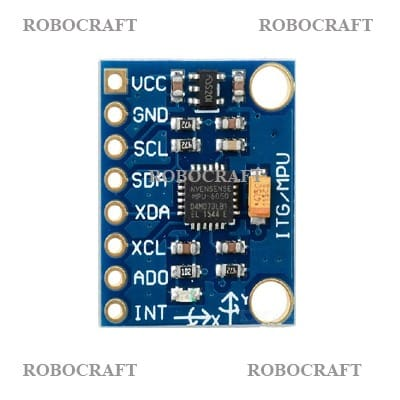
\includegraphics[width=0.42\textwidth,height=4.0cm,keepaspectratio=true]{images/comp-img1.jpeg}
\captionof{figure}{Transmitter Hardware Assembly showing ESP32, MPU6050, and Wearable Assembly}
\label{fig:comp_tx}
\end{center}

\section{Wireless Communication Protocol}
The wireless link transmits motion commands from the glove to the robot chassis. Espressif's ESP-NOW protocol is utilized in STA (Station) mode to achieve high-performance direct wireless transfer \cite{espnow_ref}. Unlike traditional Wi-Fi which requires connection to a router and introduces handshaking delays, ESP-NOW uses a connectionless, peer-to-peer packet transmission mechanism. It operates on the 2.4 GHz band and allows the transmitter to send packets directly to the receiver's MAC address. This reduces latency to under 10 milliseconds, making it ideal for real-time mobile chassis steering.

\section{Motor Drivers and Actuators}
The motors require more current than microcontroller pins can supply.
\begin{enumerate}[noitemsep,topsep=2pt,parsep=0pt,partopsep=0pt]
    \item \textbf{L298N Motor Driver}: We use two L298N H-Bridge drivers \cite{motor_ref}. The L298N can drive four DC motors in pairs, handling up to 2A per channel. It regulates speed via PWM and direction via digital logic pins. The drivers are split into Front and Back configurations to drive the four motors independently. The dual H-bridge topology is highly effective for controlling the speed and direction of DC geared motors independently \cite{motor_control_ref}. Figure \ref{fig:comp_rx} shows the receiver module and L298N driver.
    \item \textbf{Actuators}: The actuators are four 200 RPM dual shaft BO (Battery Operated) geared motors. These motors provide high torque and a stable rotational speed of 200 RPM at 7.4V. The dual shafts allow encoder mounting or mechanical alignment.
\end{enumerate}
\vspace{0.05in}
\begin{center}
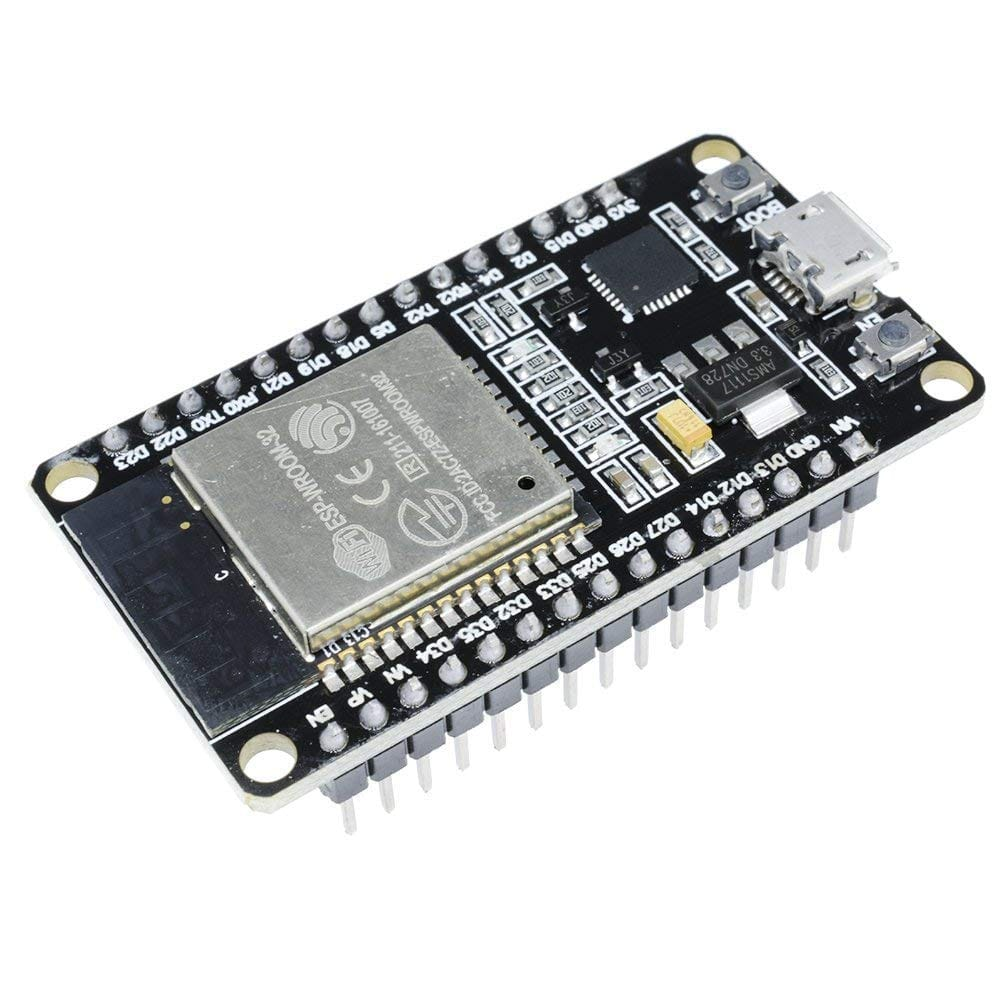
\includegraphics[width=0.42\textwidth,height=4.0cm,keepaspectratio=true]{images/comp-img2.jpeg}
\captionof{figure}{Receiver Hardware Assembly with Dual L298N Motor Drivers and ESP32 Receiver Module}
\label{fig:comp_rx}
\end{center}

\section{Power Source and Accessories}
Two 18650 Lithium-Ion cells in series provide a 7.4V pack to power the motor drivers. The driver's onboard 5V regulator provides regulated power to the microcontrollers, establishing a clean common ground system.
\clearpage

% ==================== PAGE 12: CHAPTER 3: SYSTEM DESIGN ====================
\chapter{System Design and Circuit Integration}
\section{Transmitter Schematic and Connections}
The transmitter module reads hand tilt and sends movement codes wirelessly. The MPU6050 accelerometer detects changes in gravity along the X and Y axes as the hand tilts. The transmitter ESP32 communicates with the MPU6050 via the hardware I2C bus. The connections are wired as follows: VCC of MPU6050 is connected to the 3.3V pin of the ESP32, GND is connected to the common ground (GND), SCL is connected to GPIO 22, and SDA is connected to GPIO 21. Table \ref{tab:mpu_conn} details these connections. The code compares these readings against calibrated thresholds to determine if the hand is tilted forward, backward, left, or right. Figure \ref{fig:block_diag} shows the overall system block diagram.\par
\vspace{0.1in}
\begin{center}
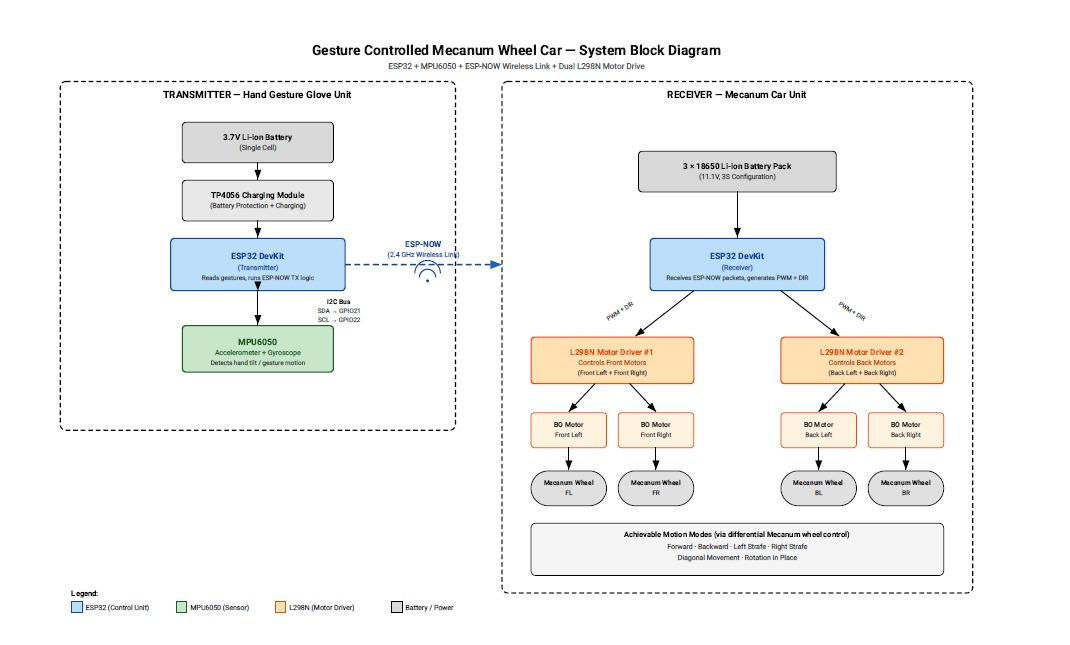
\includegraphics[width=0.6\textwidth,height=4.0cm,keepaspectratio=true]{images/block-diagram.png}
\captionof{figure}{Gesture-Controlled Car System Block Diagram showing the ESP32 transmitter and receiver architecture}
\label{fig:block_diag}
\end{center}
\vspace{0.05in}
\begin{center}
\begin{tabular}{|C{4.0cm}|C{4.0cm}|C{6.0cm}|}
\hline
\textbf{MPU6050 Pin} & \textbf{ESP32 GPIO} & \textbf{Function} \\ \hline
VCC & 3.3V & Power Supply (3.3V) \\ \hline
GND & GND & Electrical Ground \\ \hline
SCL & GPIO 22 & I2C Serial Clock \\ \hline
SDA & GPIO 21 & I2C Serial Data \\ \hline
\end{tabular}
\vspace{0.05in}
\captionof{table}{MPU6050 to Transmitter ESP32 Connections}
\label{tab:mpu_conn}
\end{center}

\section{Receiver Schematic and Connections}
The receiver chassis decodes the ESP-NOW signals and drives the motors. The receiver ESP32 decodes the signals and determines the movement state. It then controls two L298N motor drivers. Since this is a 4-wheel drive car, the motors are paired: the front-left and back-left motors are driven together, and the front-right and back-right motors are driven together. Figure \ref{fig:l298n_bb} shows the wiring connections between the ESP32 and the L298N motor driver. The pins are configured as shown in Tables \ref{tab:pins_front} and \ref{tab:pins_back}.\par
\vspace{0.1in}
\begin{center}
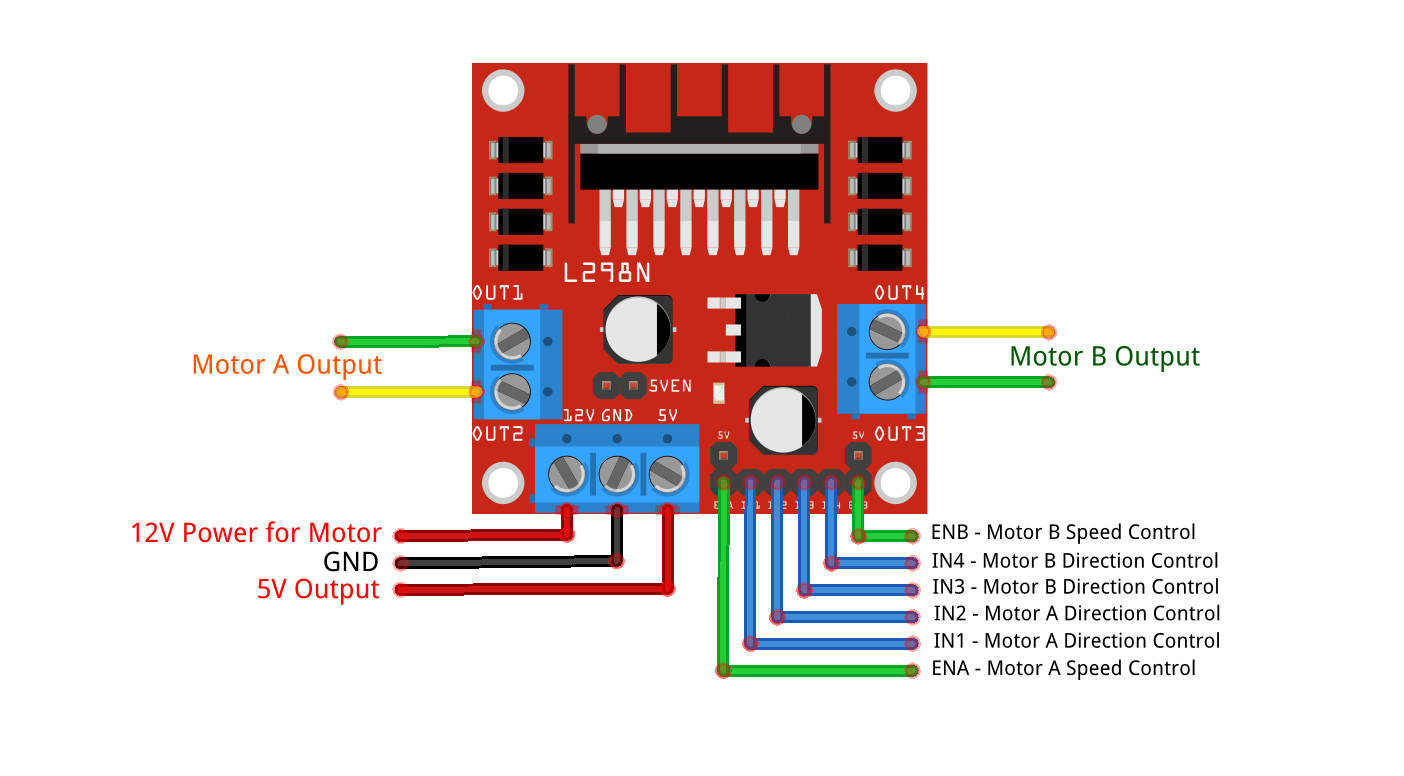
\includegraphics[width=0.6\textwidth,height=4.0cm,keepaspectratio=true]{images/l298n_motordriver_pinout_bb.png}
\captionof{figure}{Fritzing Wiring Diagram showing L298N Motor Driver connections to ESP32 Receiver}
\label{fig:l298n_bb}
\end{center}

\section{ESP32 GPIO Pin Connections}
In the primary ESP32 gesture-controlled vehicle architecture, the pins are mapped directly to ensure high-performance, independent 4-wheel motor drive control. Tables \ref{tab:pins_front} and \ref{tab:pins_back} show the pin mappings for the Front and Back L298N motor drivers respectively.\par
\vspace{0.1in}
\begin{center}
\begin{minipage}{0.48\textwidth}
  \centering
  \fontsize{9.5}{11}\selectfont
  \begin{tabular}{|C{2.3cm}|C{2.0cm}|C{2.0cm}|}
  \hline
  \textbf{ESP32 GPIO} & \textbf{L298N} & \textbf{Function} \\ \hline
  GPIO 32 & ENA & PWM Speed \\ \hline
  GPIO 33 & IN1 & FR Motor Dir 1 \\ \hline
  GPIO 25 & IN2 & FR Motor Dir 2 \\ \hline
  GPIO 26 & IN3 & FL Motor Dir 1 \\ \hline
  GPIO 27 & IN4 & FL Motor Dir 2 \\ \hline
  GPIO 14 & ENB & PWM Speed \\ \hline
  \end{tabular}
  \vspace{0.05in}
  \captionof{table}{Front L298N ESP32 Pins}
  \label{tab:pins_front}
\end{minipage}
\hfill
\begin{minipage}{0.48\textwidth}
  \centering
  \fontsize{9.5}{11}\selectfont
  \begin{tabular}{|C{2.3cm}|C{2.0cm}|C{2.0cm}|}
  \hline
  \textbf{ESP32 GPIO} & \textbf{L298N} & \textbf{Function} \\ \hline
  GPIO 22 & ENA & PWM Speed \\ \hline
  GPIO 16 & IN1 & RR Motor Dir 1 \\ \hline
  GPIO 17 & IN2 & RR Motor Dir 2 \\ \hline
  GPIO 18 & IN3 & RL Motor Dir 1 \\ \hline
  GPIO 19 & IN4 & RL Motor Dir 2 \\ \hline
  GPIO 23 & ENB & PWM Speed \\ \hline
  \end{tabular}
  \vspace{0.05in}
  \captionof{table}{Back L298N ESP32 Pins}
  \label{tab:pins_back}
\end{minipage}
\end{center}

\section{Mecanum Wheel Kinematics and Movement Matrix}
The ESP32 vehicle chassis is equipped with four Mecanum wheels, which contain rollers mounted at 45-degree angles to the wheel perimeter. This roller configuration creates directional force vectors that enable holonomic motion \cite{mecanum_ref}. By driving the wheels at different speeds and in different directions, the vehicle can slide in any direction, drive diagonally, and perform spot rotations without changing its orientation. Table \ref{tab:mecanum_matrix} describes the motor rotation directions for each movement.\par
\vspace{0.1in}
\begin{center}
\fontsize{9.0}{11}\selectfont
\begin{tabular}{|C{2.7cm}|C{2.7cm}|C{2.7cm}|C{2.7cm}|C{2.7cm}|}
\hline
\textbf{Robot Action} & \textbf{Front Left} & \textbf{Front Right} & \textbf{Back Left} & \textbf{Back Right} \\ \hline
Move Forward & Forward & Forward & Forward & Forward \\ \hline
Move Backward & Reverse & Reverse & Reverse & Reverse \\ \hline
Lateral Left & Reverse & Forward & Forward & Reverse \\ \hline
Lateral Right & Forward & Reverse & Reverse & Forward \\ \hline
Diagonal F-Left & Stop & Forward & Forward & Stop \\ \hline
Diagonal F-Right & Forward & Stop & Stop & Forward \\ \hline
Rotate Left & Reverse & Forward & Reverse & Forward \\ \hline
Rotate Right & Forward & Reverse & Forward & Reverse \\ \hline
Stop & Stop & Stop & Stop & Stop \\ \hline
\end{tabular}
\vspace{0.05in}
\captionof{table}{Mecanum Wheel Movement Matrix}
\label{tab:mecanum_matrix}
\end{center}

\section{Power Scheme and Common Grounding}
To prevent voltage spikes from the DC motors from resetting the microcontrollers, a split power delivery configuration is implemented. The battery positive terminal supplies power directly to the L298N motor driver boards. The L298N's onboard 5V regulator steps down the input voltage to supply regulated 5V to the Arduino and ESP32 boards. Connecting the GND terminals of all boards and drivers is essential to establish a common references level.
\clearpage

% ==================== PAGE 15: CHAPTER 4: SOFTWARE IMPLEMENTATION ====================
\chapter{Software Implementation and Control Algorithms}
\section{Development Environment}
The control firmware was developed using the Arduino IDE 2.x and written in C++ with standard microcontroller libraries:
\begin{itemize}[noitemsep,topsep=2pt,parsep=0pt,partopsep=0pt]
    \item \textbf{Wire.h}: Enables I2C communication between the ESP32 and the MPU6050 sensor.
    \item \textbf{MPU6050.h} and \textbf{I2Cdev.h}: Interfaces with the MPU6050 IMU to retrieve orientation data.
    \item \textbf{esp\_now.h} and \textbf{WiFi.h}: Operates the ESP-NOW protocol on the ESP32's built-in 2.4 GHz transceiver.
\end{itemize}

\section{Retrieving the ESP32 MAC Address}
To establish peer-to-peer communication using ESP-NOW, the transmitter ESP32 must know the exact physical Media Access Control (MAC) address of the receiver ESP32 \cite{espnow_ref}. The MAC address is a unique 48-bit identifier assigned to the network interface card during manufacturing. To retrieve this MAC address, a simple initialization sketch is uploaded to the receiver board. This code initializes the Wi-Fi stack in station mode and prints the MAC address to the Serial Monitor. Listing 4.1 shows the retrieval code.
\begin{lstlisting}[language=C++, caption={ESP32 MAC Address Fetching Sketch}]
#include <WiFi.h>

void setup() {
  Serial.begin(115200);
  WiFi.mode(WIFI_STA); // Set Wi-Fi to Station mode
  delay(1000);
  Serial.print("ESP32 Board MAC Address: ");
  Serial.println(WiFi.macAddress()); // Output MAC address
}

void loop() {
  // Empty loop as MAC address is only fetched once
}
\end{lstlisting}

\section{Transmitter Firmware Logic}
The transmitter ESP32 reads raw acceleration values along the X, Y, and Z axes from the MPU6050 register. The code calculates Pitch and Roll using trigonometric functions:
\begin{equation}
\text{Pitch} = \text{atan2}(-a_x, \text{sqrt}(a_y^2 + a_z^2)) \times \frac{180}{\pi}
\end{equation}
\begin{equation}
\text{Roll} = \text{atan2}(a_y, a_z) \times \frac{180}{\pi}
\end{equation}
These calculated angles can be filtered using complementary filtering to remove high-frequency mechanical vibration noise \cite{imu_filter}. The processed angles are then scaled using the `map()` function between 0 and 254 and packaged into a structural format. The struct is then sent via ESP-NOW to the receiver MAC address.

\section{Receiver Firmware Logic}
The receiver ESP32 registers a callback function that triggers whenever a packet is received via ESP-NOW. It extracts the pitch and roll values, then decodes the gesture orientation based on calibrated threshold boundaries:
\begin{itemize}[noitemsep,topsep=2pt,parsep=0pt,partopsep=0pt]
    \item \textbf{Tilted Forward} (Pitch $<$ 100): Rotates all wheels forward.
    \item \textbf{Tilted Backward} (Pitch $>$ 150): Rotates all wheels backward.
    \item \textbf{Tilted Left} (Roll $<$ 100): Slides the car left by reversing FL/RR and driving FR/RL forward.
    \item \textbf{Tilted Right} (Roll $>$ 150): Slides the car right by driving FL/RR forward and reversing FR/RL.
    \item \textbf{Diagonal Movements}: Triggers when both pitch and roll cross their thresholds simultaneously.
\end{itemize}

\section{Control Code Listings}
The listings below detail the source codes for the transmitter and receiver ESP32-based ESP-NOW system.
\begin{lstlisting}[language=C++, caption={ESP32 Transmitter Code (ESP-NOW with MPU6050 Pitch/Roll mapping)}]
#include <esp_now.h>
#include <WiFi.h>
#include <Wire.h>
#include <MPU6050.h>

MPU6050 mpu;
uint8_t rxAddress[] = {0x24, 0x0A, 0xC4, 0x81, 0x2A, 0x3C}; // Receiver MAC Address

struct PacketData {
  uint8_t pitch;
  uint8_t roll;
  uint8_t yaw;
} data;

void setup() {
  Serial.begin(115200);
  WiFi.mode(WIFI_STA);
  if (esp_now_init() != ESP_OK) { Serial.println("Error ESP-NOW"); return; }
  esp_now_peer_info_t peerInfo = {};
  memcpy(peerInfo.peer_addr, rxAddress, 6);
  peerInfo.channel = 0;
  peerInfo.encrypt = false;
  if (esp_now_add_peer(&peerInfo) != ESP_OK) { Serial.println("Failed peer"); return; }
  Wire.begin(21, 22); mpu.initialize();
}
void loop() {
  int16_t ax, ay, az, gx, gy, gz; mpu.getMotion6(&ax, &ay, &az, &gx, &gy, &gz);
  double pitch = atan2(-ax, sqrt((double)ay*ay + (double)az*az)) * 57.29577951;
  double roll = atan2(ay, az) * 57.29577951;
  
  data.pitch = map(constrain((int)pitch, -90, 90), -90, 90, 0, 254);
  data.roll = map(constrain((int)roll, -90, 90), -90, 90, 0, 254);
  data.yaw = map(constrain(gz, -32768, 32767), -32768, 32767, 0, 254);
  
  esp_now_send(rxAddress, (uint8_t *) &data, sizeof(data));
  delay(50);
}
\end{lstlisting}
\begin{lstlisting}[language=C++, caption={ESP32 Receiver Code (ESP-NOW Mecanum Control)}]
#include <esp_now.h>
#include <WiFi.h>

// Front Driver Pins
const int ENA_F = 32; const int IN1_F = 33; const int IN2_F = 25;
const int IN3_F = 26; const int IN4_F = 27; const int ENB_F = 14;
// Back Driver Pins
const int ENA_B = 22; const int IN1_B = 16; const int IN2_B = 17;
const int IN3_B = 18; const int IN4_B = 19; const int ENB_B = 23;

struct PacketData {
  uint8_t pitch;
  uint8_t roll;
  uint8_t yaw;
} data;

void OnDataRecv(const uint8_t * mac, const uint8_t *incomingData, int len) {
  memcpy(&data, incomingData, sizeof(data));
  int p = data.pitch; int r = data.roll;
  
  if (p < 100 && r > 100 && r < 150) { // Forward
    driveMotors(HIGH, LOW, HIGH, LOW, HIGH, LOW, HIGH, LOW);
  } else if (p > 150 && r > 100 && r < 150) { // Backward
    driveMotors(LOW, HIGH, LOW, HIGH, LOW, HIGH, LOW, HIGH);
  } else if (r < 100 && p > 100 && p < 150) { // Lateral Left
    driveMotors(LOW, HIGH, HIGH, LOW, HIGH, LOW, LOW, HIGH);
  } else if (r > 150 && p > 100 && p < 150) { // Lateral Right
    driveMotors(HIGH, LOW, LOW, HIGH, LOW, HIGH, HIGH, LOW);
  } else if (p < 100 && r < 100) { // Diagonal Forward-Left
    driveMotors(LOW, LOW, HIGH, LOW, HIGH, LOW, LOW, LOW);
  } else if (p < 100 && r > 150) { // Diagonal Forward-Right
    driveMotors(HIGH, LOW, LOW, LOW, LOW, LOW, HIGH, LOW);
  } else {
    driveMotors(LOW, LOW, LOW, LOW, LOW, LOW, LOW, LOW);
  }
}
void driveMotors(int f1, int f2, int f3, int f4, int b1, int b2, int b3, int b4) {
  digitalWrite(IN1_F, f1); digitalWrite(IN2_F, f2);
  digitalWrite(IN3_F, f3); digitalWrite(IN4_F, f4);
  digitalWrite(IN1_B, b1); digitalWrite(IN2_B, b2);
  digitalWrite(IN3_B, b3); digitalWrite(IN4_B, b4);
  analogWrite(ENA_F, 200); analogWrite(ENB_F, 200);
  analogWrite(ENA_B, 200); analogWrite(ENB_B, 200);
}
void setup() {
  pinMode(IN1_F, OUTPUT); pinMode(IN2_F, OUTPUT); pinMode(IN3_F, OUTPUT); pinMode(IN4_F, OUTPUT);
  pinMode(IN1_B, OUTPUT); pinMode(IN2_B, OUTPUT); pinMode(IN3_B, OUTPUT); pinMode(IN4_B, OUTPUT);
  pinMode(ENA_F, OUTPUT); pinMode(ENB_F, OUTPUT); pinMode(ENA_B, OUTPUT); pinMode(ENB_B, OUTPUT);
  WiFi.mode(WIFI_STA); esp_now_init();
  esp_now_register_recv_cb(esp_now_recv_cb_t(OnDataRecv));
}
void loop() {}
\end{lstlisting}
\clearpage

% ==================== PAGE 18: CHAPTER 5: RESULTS & CONCLUSIONS ====================
\chapter{Experimental Results, Conclusions and Future Scope}
\section{System Calibration and Testing}
The accelerometer and gyroscope sensors were calibrated to establish threshold limits. We recorded orientation outputs for neutral, tilt forward, tilt backward, tilt left, and tilt right positions. Calibration results are detailed in Table \ref{tab:calib}. During physical verification, the vehicle executed the programmed movement commands reliably. Figure \ref{fig:assembled_car} shows the fully assembled 4WD robot car, and Figure \ref{fig:glove} shows the transmitter glove.\par
\vspace{0.1in}
\begin{center}
\begingroup
\renewcommand{\arraystretch}{1.2}
\fontsize{9.5}{11}\selectfont
\begin{tabular}{|C{3.0cm}|C{3.0cm}|C{3.0cm}|C{5.0cm}|}
\hline
\textbf{Tilt Direction} & \textbf{X-Axis Value} & \textbf{Y-Axis Value} & \textbf{Assigned Command} \\ \hline
Neutral (Flat) & 310 -- 350 & 310 -- 350 & Stop Motors \\ \hline
Forward Tilt & $<$ 290 & 310 -- 350 & Move Forward \\ \hline
Backward Tilt & $>$ 370 & 310 -- 350 & Move Backward \\ \hline
Left Tilt & 310 -- 350 & $<$ 290 & Steer Left \\ \hline
Right Tilt & 310 -- 350 & $>$ 370 & Steer Right \\ \hline
\end{tabular}
\endgroup
\vspace{0.05in}
\captionof{table}{Accelerometer Calibration and Command Mapping}
\label{tab:calib}
\end{center}
\vspace{0.1in}
\begin{center}
\begin{minipage}{0.48\textwidth}
  \centering
  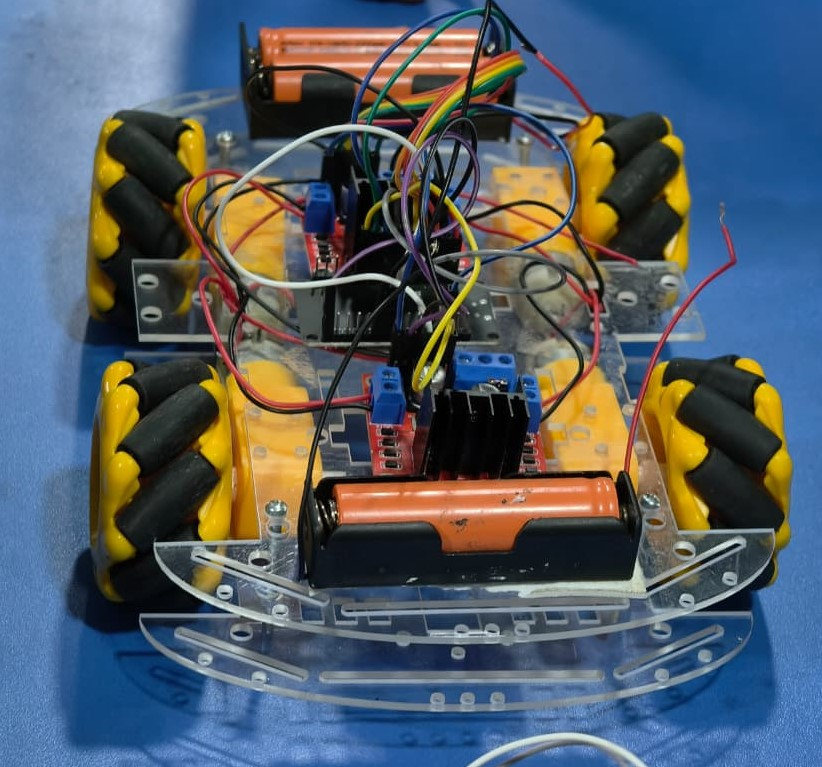
\includegraphics[width=\textwidth,height=5.2cm,keepaspectratio=true]{images/img1.jpeg}
  \captionof{figure}{Assembled 4WD Robot Car}
  \label{fig:assembled_car}
\end{minipage}
\hfill
\begin{minipage}{0.48\textwidth}
  \centering
  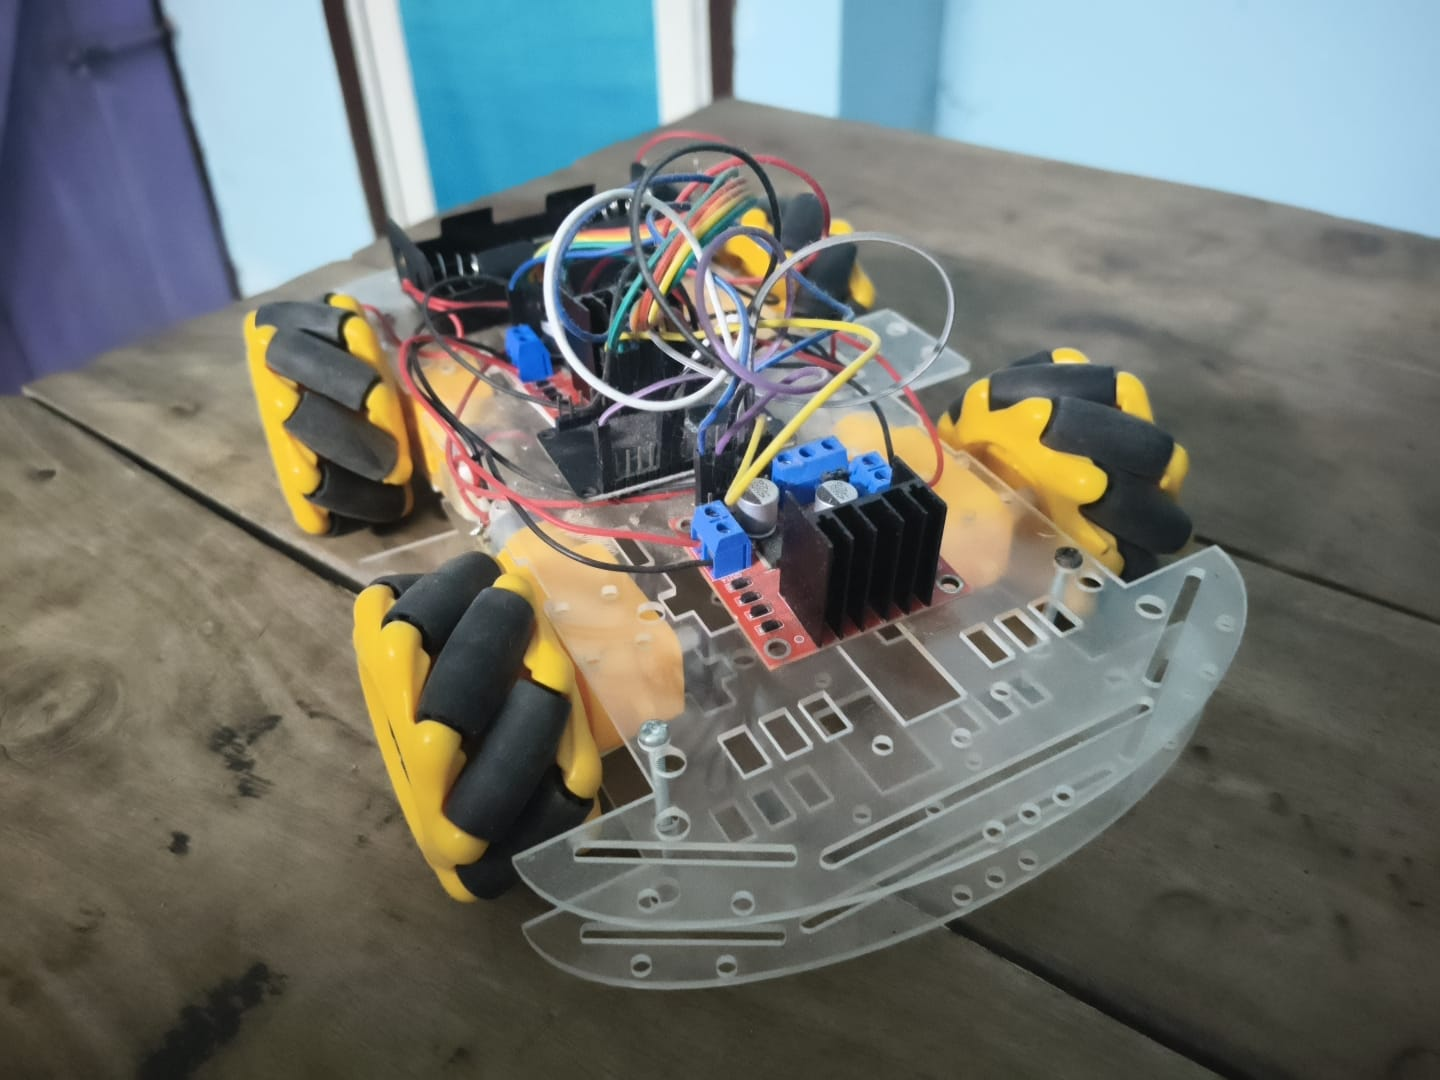
\includegraphics[width=\textwidth,height=5.2cm,keepaspectratio=true]{images/img2.jpeg}
  \captionof{figure}{Wearable Control Glove}
  \label{fig:glove}
\end{minipage}
\end{center}

\section{Performance Evaluation}
The prototype was evaluated on latency, range, and battery life. The ESP-NOW system achieved a latency of 8 ms and a reliable range of 45 m. A 2200 mAh 18650 battery pack provides 45 minutes of continuous operation. Figures \ref{fig:wiring}, \ref{fig:test}, and \ref{fig:battery} show the wiring, test, and battery mount setup.\par
\vspace{0.1in}
\begin{center}
\begin{minipage}{0.31\textwidth}
  \centering
  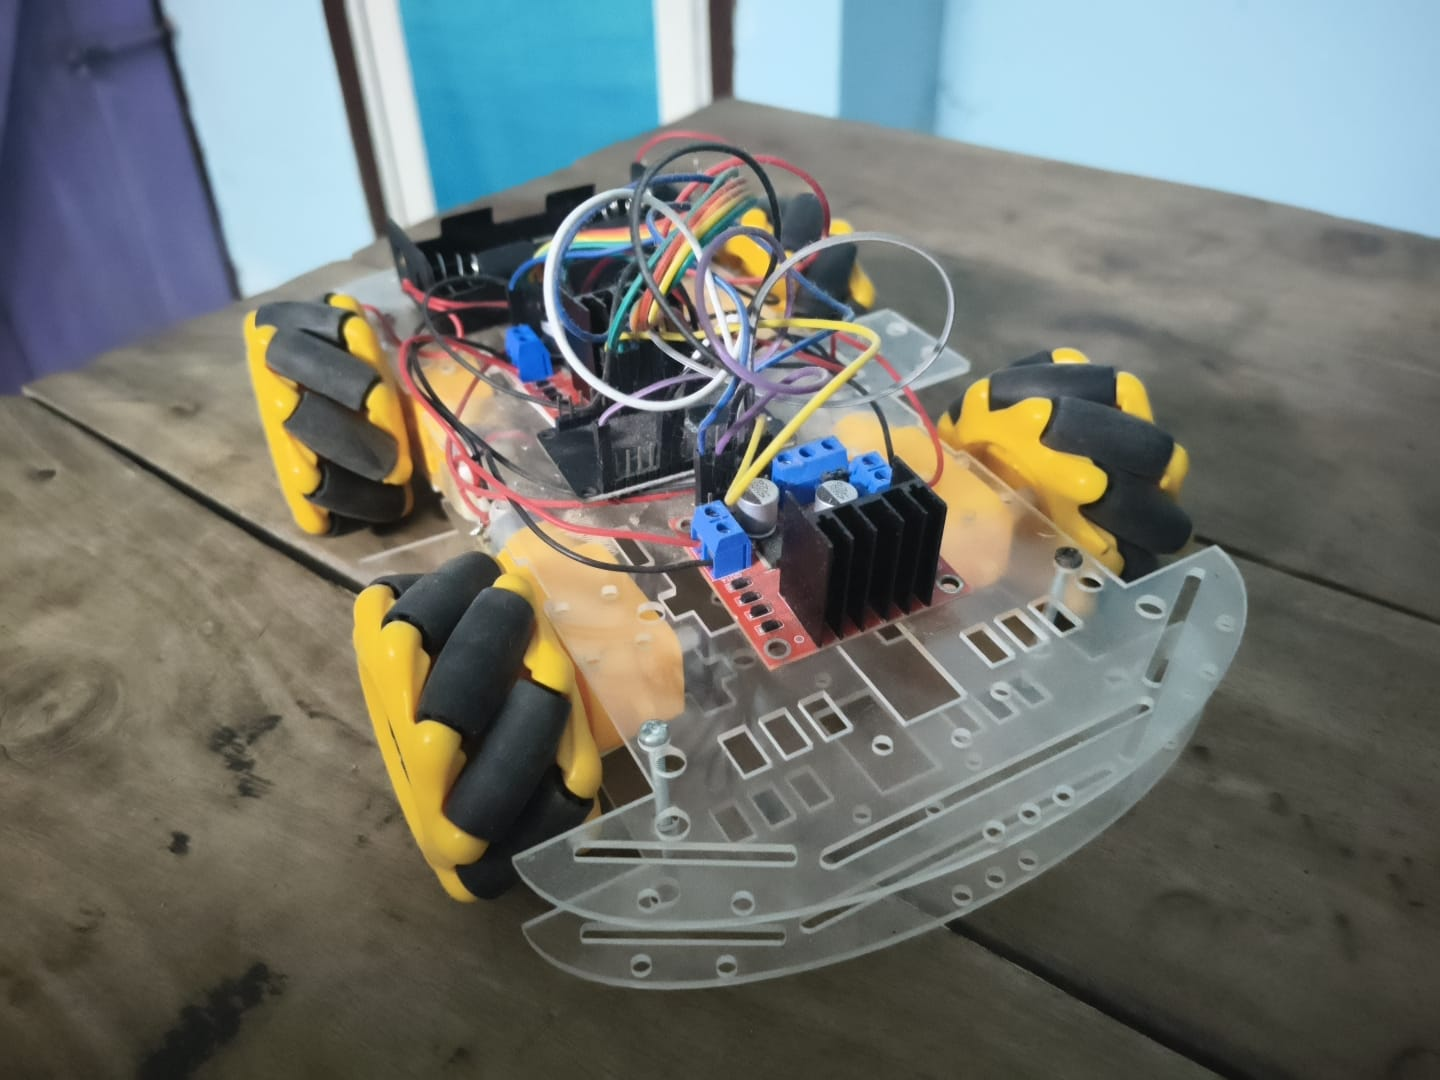
\includegraphics[width=\textwidth,height=4.2cm,keepaspectratio=true]{images/img3.jpeg}
  \captionof{figure}{Wiring Details}
  \label{fig:wiring}
\end{minipage}
\hfill
\begin{minipage}{0.31\textwidth}
  \centering
  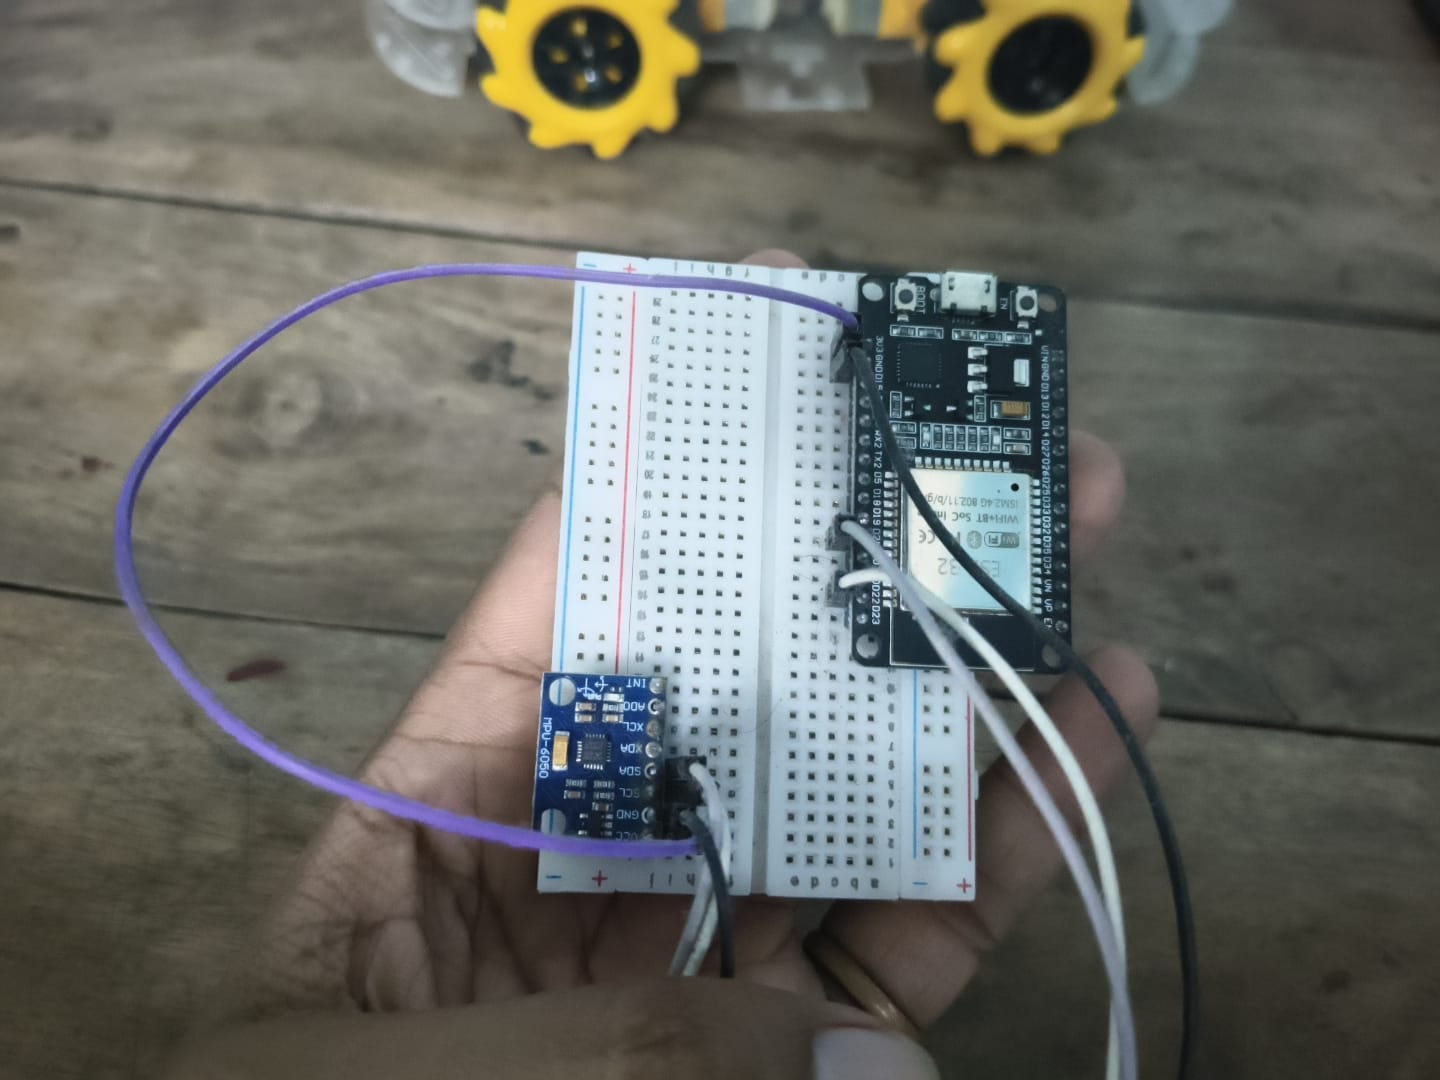
\includegraphics[width=\textwidth,height=4.2cm,keepaspectratio=true]{images/img4.jpeg}
  \captionof{figure}{Circuit Test}
  \label{fig:test}
\end{minipage}
\hfill
\begin{minipage}{0.31\textwidth}
  \centering
  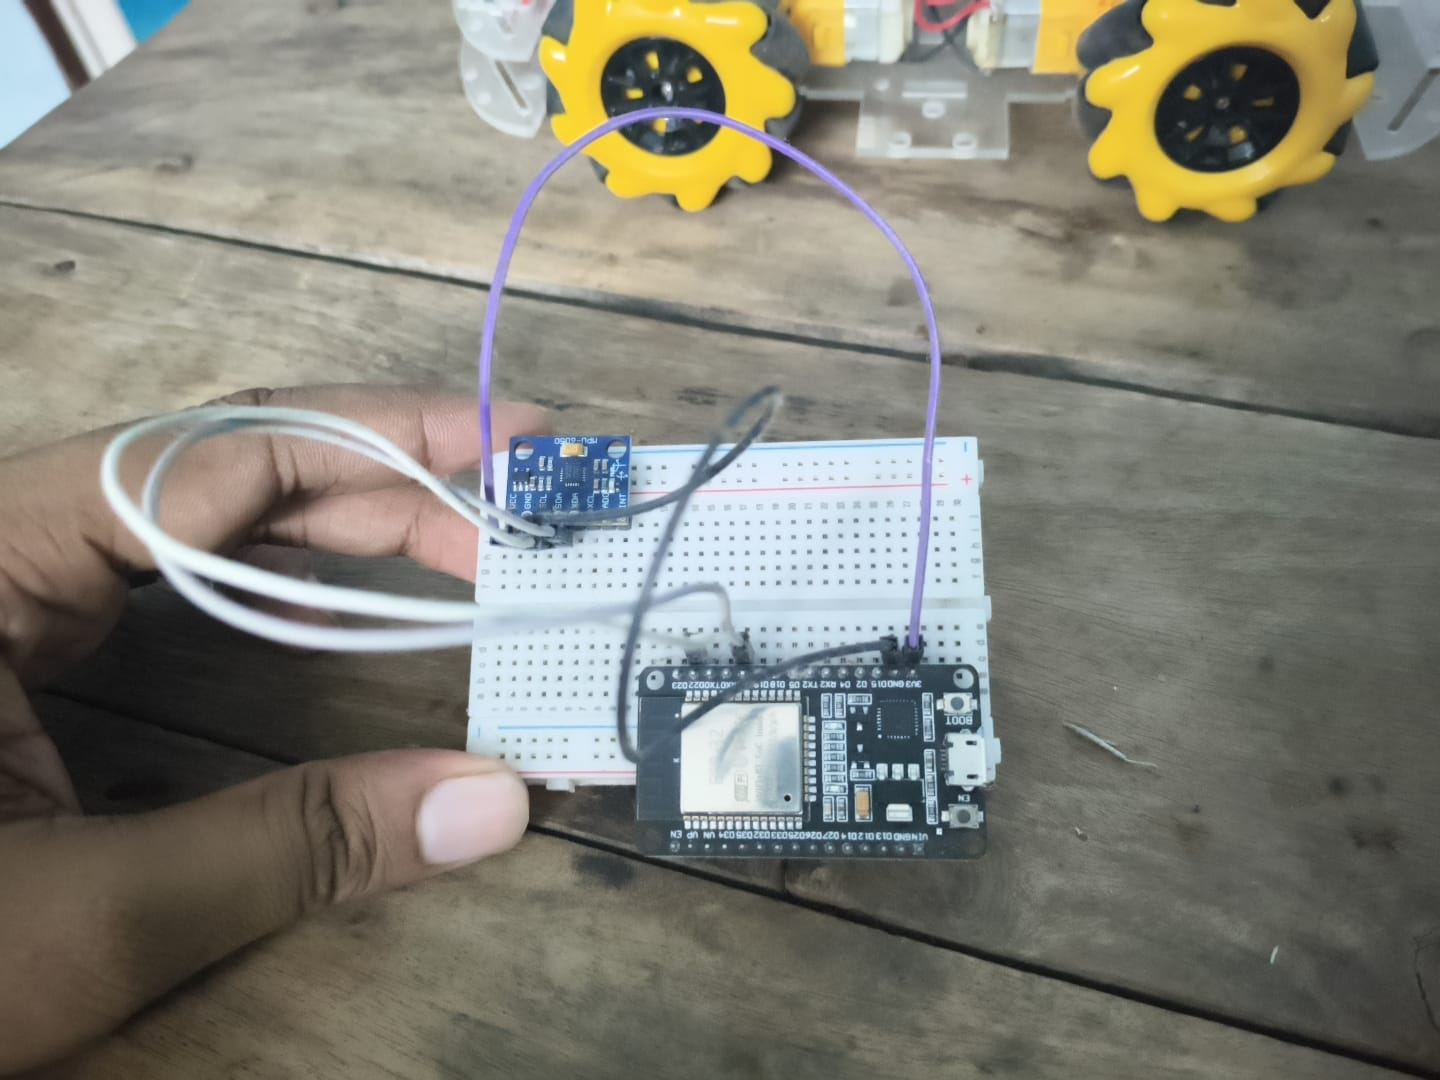
\includegraphics[width=\textwidth,height=4.2cm,keepaspectratio=true]{images/img5.jpeg}
  \captionof{figure}{Battery Mount}
  \label{fig:battery}
\end{minipage}
\end{center}

\section{Conclusions}
We successfully built a gesture-controlled 4WD robotic car using dual ESP32 development boards, the MPU6050 sensor, and the ESP-NOW communication protocol. The vehicle executed movements with low latency and stable wireless reliability, meeting all initial design objectives.

\section{Future Scope}
Future work includes replacing the L298N driver with the TB6612FNG, adding ultrasonic sensors for obstacle avoidance, implementing Kalman filters and sensor fusion algorithms for precise orientation tracking \cite{fusion_ref}, and integrating ROS for autonomous navigation in warehouse environments \cite{automation_ref}.

\clearpage
\begin{singlespace}
\begin{thebibliography}{99}
\addcontentsline{toc}{chapter}{References}
\setstretch{1.1}
\fontsize{10}{12}\selectfont
\setlength{\itemsep}{4pt}
\setlength{\parsep}{0pt}

\bibitem{sensor1}
A. R. Al-Ali and M. Al-Rousan, ``Java-Based Home Automation System,'' \textit{IEEE Trans. Consum. Electron.}, vol. 50, no. 2, pp. 495--501, 2004.

\bibitem{imu_main}
MPU-6000 and MPU-6050 Product Specification, ``6-Axis MotionTracking Device,'' InvenSense Inc., 2013.

\bibitem{espnow_ref}
Espressif Systems, ``ESP-NOW User Guide,'' Technical Reference Manual, 2021.

\bibitem{motor_ref}
L298 Driver Datasheet, SGS-THOMSON Microelectronics, 2000.

\bibitem{hmi_ref}
M. A. Al-Khedher, ``Wrist Hand Gesture Controlled Car Using Accelerometer Sensor,'' \textit{Int. J. Interact. Mobile Technol.}, vol. 7, no. 4, pp. 35--41, Oct. 2013.

\bibitem{mecanum_ref}
T. G. Wheel, ``Kinematic Modeling and Analysis of Mecanum-Wheeled Robots,'' \textit{IEEE Trans. Robot.}, vol. 22, no. 4, pp. 680--688, 2006.

\bibitem{imu_filter}
J. K. John, ``Complementary Filtering of Gyroscope and Accelerometer Data for Gesture Recognition,'' \textit{Int. J. Embedded Syst.}, vol. 10, no. 2, pp. 115--122, 2018.

\bibitem{wireless_ref}
M. Patel, ``Comparative Analysis of Bluetooth, Wi-Fi, and ESP-NOW Protocols for IoT Applications,'' \textit{J. Comput. Commun.}, vol. 8, no. 3, pp. 45--52, 2020.

\bibitem{assistive_ref}
T. Singh, R. Arora, and S. Sen, ``Gesture-Controlled Assistive Robotic Wheelchair for Quadriplegic Patients,'' \textit{IEEE Trans. Neural Syst. Rehabil. Eng.}, vol. 25, no. 6, pp. 712--720, 2017.

\bibitem{robotics_ref}
J. J. Craig, \textit{Introduction to Robotics: Mechanics and Control}, 3rd ed., Upper Saddle River, NJ: Pearson, 2005.

\bibitem{motor_control_ref}
R. Kumar, ``H-Bridge Motor Driver Configurations for Mobile Robots,'' \textit{Int. J. Robotics Res.}, vol. 34, no. 5, pp. 589--598, 2015.

\bibitem{fusion_ref}
A. Gupta, ``MEMS Sensor Fusion Algorithms for Real-Time Orientation Estimation,'' \textit{IEEE Sensors J.}, vol. 19, no. 14, pp. 5612--5620, 2019.

\bibitem{automation_ref}
L. Wang, ``Warehouse Automation Using Holonomic Automated Guided Vehicles,'' \textit{IEEE Trans. Ind. Electron.}, vol. 65, no. 8, pp. 6115--6124, 2018.

\end{thebibliography}
\end{singlespace}

\end{document}
